\documentclass[twoside,12pt]{article}
\usepackage{indentfirst}
\usepackage{bm}    %%%%%  排印数学符号黑斜体时调用此宏包
\usepackage{verbatim} %% 抄录环境宏包,本模板文件使用
\usepackage{graphicx}
\usepackage{epsf}
\usepackage{caption2}
%%\usepackage{epsfig} %%% 文中插入 eps 图形时也可调用此宏包,插图方法 2
%%\usepackage{amsmath}  %%% 排印比较复杂的数学公式和符号时可调用此宏包
%\usepackage[T1]{fontenc}
%%% 因为物理学报的参考文献不需要节标题,需重新定义参考文献环境指令
\makeatletter
\newdimen\bibindent
\setlength\bibindent{1.5em}
\renewenvironment{thebibliography}[1]
     {\list{\@biblabel{\@arabic\c@enumiv}}%
           {\settowidth\labelwidth{\@biblabel{#1}}%
            \leftmargin\labelwidth
            \advance\leftmargin\labelsep
            \@openbib@code
            \usecounter{enumiv}%
            \let\p@enumiv\@empty
            \renewcommand\theenumiv{\@arabic\c@enumiv}}%
      \sloppy
      \clubpenalty4000
      \@clubpenalty \clubpenalty
      \widowpenalty4000%
      \sfcode`\.\@m}
     {\def\@noitemerr
       {\@latex@warning{Empty `thebibliography' environment}}%
      \endlist}
\makeatother
%%%%%%%%%% APS 要求的部分宏命令和页面参数设置
\renewcommand{\baselinestretch}{1.5}     %% 正文行距参数设置
%%%%%%%%%% 正文一级、二级、三级标题的序号设置
\renewcommand{\thesection}{\arabic{section}.\hspace{-.4cm}}
\renewcommand{\thesubsection}{\arabic{section}.\arabic{subsection}.\hspace{-.4cm}}
\renewcommand{\thesubsubsection}{\arabic{section}.\arabic{subsection}.\arabic{subsubsection}.\hspace{-.3cm}}
%%%%%%%%%%%%%%%%%%%%%%%%页面参数设置
\footskip=20pt  \headsep=2truemm \topmargin=0cm \oddsidemargin=0pt \evensidemargin=0pt
\textwidth=170truemm   %% 页面宽度
\textheight=245truemm  %% 页面高度
\parindent=20pt        %% 段缩进
% \def\thefootnote{}  %% 去掉脚注序号标号
\def\thefootnote{\fnsymbol{footnote}}  %% 使用符号型脚注序号
%%%%%%%%%%%%%%%%%%%%%%%%%%%%%%%
\baselineskip=14pt plus.2pt minus.2pt
\parskip=0pt plus.1pt minus.1pt
\abovedisplayskip=8pt plus.2pt minus.2pt
\belowdisplayskip=8pt plus.2pt minus.2pt

\usepackage{xeCJK}
%\usepackage{fontspec}
\setCJKmainfont[BoldFont=simhei.ttf]{simsun.ttf}
\setCJKsansfont{simhei.ttf}
\setCJKmonofont{simfang.ttf}

%\setCJKmainfont{Adobe Song Std}
%\setCJKmainfont[BoldFont=Adobe Heiti Std]{Adobe Song Std}
%%%%%%%%%%%%%%%%%%%%%%%%%%%%%%%%%%%%%%%%%%%%%%%%%%%%%%

\begin{document}    %% 文本文件开始,这是必须的指令
\def\sectionformat{\normalfont\Large} %% 2011-5-2
\def\subsectionformat{\normalfont\large}
\def\subsubsectionformat{\normalfont\normalsize}
%-------------------  First Head  -----------------------------------------
\thispagestyle{empty} \vspace*{0.8cm}\hbox
to\textwidth{\vbox{\hfill\huge\sf Acta Physica Sinica\hfill}}
\par\noindent\rule[3mm]{\textwidth}{0.2pt}\hspace*{-\textwidth}\noindent
\rule[2.5mm]{\textwidth}{0.2pt}

%=================== Text begin here =============================================
\renewcommand\figurename{\small 图}
\renewcommand{\captionlabeldelim}{~}


\begin{center}
\Large 微通道中高分子运动的耗散粒子动力学模拟$^{*}$
\end{center}

\begin{center}
{ 周吕文-1$^{1)}$ \ \ 刘谋斌-2$^{1,2)}$ \ \
\ 常建忠-3$^{3)}$ }
\end{center}

\begin{center}
\begin{footnotesize}
1)\ 中国科学院力学研究所水动力学与海洋工程重点实验室,北京 100190\ a) \\
2)\ 中国科学院力学研究所非线性力学国家重点实验室,北京 100190\ b) \\
3)\ 中北大学机电工程学院,太原 030051\ c)
\end{footnotesize}
\end{center}

\begin{center}
\footnotesize (XXXX XX X 收到; XXXX XX X 收到修改稿)
          %% (XXXX XX X: 年 月 日)
\end{center}

\vspace*{2mm}

\begin{center}
\begin{minipage}{15.5cm}
\parindent 20pt\footnotesize
了解高分子在微通道内的流动行为对于生物和医学方面的研究与应用具有重要的意义。
在高分子的输运与迁移过程中,微通道的宽度往往与高分子的长度在同一个量级上,传
统连续介质力学理论不一定适用。利用耗散粒子动力学及有限拉伸非线性弹性珠簧链
模型,对不同数量,不同长度的高分子链在直通道及微缩通道中的流动进行了模拟与
分析。研究表明,高分子的存在对微通道系统的温度没有明显影响,对密度与水平流
动速度有较明显的影响。高分子链直接影响到周围的简单流体粒子,降低其周围流体
粒子的流动速度,并使密度产生波动,形成``拖曳''现象。高分子链分布越密集,长度
越长,高分子链的拖曳现象越明显。
\end{minipage}
\end{center}

\begin{center}
\begin{minipage}{15.5cm}
\begin{minipage}[t]{2.3cm}{ 关键词: }\end{minipage}
\begin{minipage}[t]{13.1cm}
耗散粒子动力学,高分子,微流动
\end{minipage}\par\vglue8pt
{\bf PACS: }
47.11.j, 47.15.Rq
\end{minipage}
\end{center}

\section{ 引言}

微细加工技术的发展对环境工程、生物化学工程、医学工程等不同领域具有极其重要
的意义。生物微型器件的设计和制造可以提供更加快捷有效的手段,对疾病进行诊断、
分析及治疗。如微针可以高效而精确的对细胞、局部组织等进行微小剂量的药物或高
分子的输送。因此,了解药物或者DNA等高分子在微通道中的流动行为对于生物微型
器件的设计和制造是至关重要的。

介观尺度流动现象普遍存在于环境工程、生物化学工程和微纳米科技等不同领域,微通
道的特征尺寸与DNA高分子的长度都处于介观尺度,发展对介观尺度流动现象的模拟技术
是近年来国际计算机模拟领域的发展趋势。传统的网格方法一般基于连续介质力学假设,
当问题所涉及的空间尺度逐渐缩小到介观乃至微观时未必适用。介观尺度流动问题的研
究往往需要多尺度计算模型以研究介观乃至微观尺度的时间和空间流体动力学特征。在
微观尺度上,分子动力学(molecular dynamics,MD)方法\cite{Rapaport}通过追踪每个流体分子的位置和动量从而对整个流体系统的特性
进行准确的模拟。由于当前计算条件的限制,分子动力学模拟所涉及的时间及空间尺度还
仅限于纳秒和纳米级,很难对介观尺度以上的流动区域进行模拟。而与介观尺度流动现象
直接相关的物理特性往往处于毫秒、微米级,因此介于纳米与毫米之间的介观尺度模拟方
法是模拟介观尺度流动问题的合理选择。


耗散粒子动力学(dissipative particle dynamics, DPD)\cite{Hoogerbrugge,Groot1997}是一种适合模拟简单和复杂流体动力学和流变性能的介观尺度方法,由 Hoogerbrugge 与 Koelman首先提出,旨在解决经典分子动力学所难以解决的流体的时间和空间尺度问题。作为
一种粗粒化的分子动力学方法,DPD方法应用粒子代表一团分子或者原子,而不是单个原子或分子。
与经典分子动力学方法相比,DPD方法可以使用更大的粒子尺寸和更长的时间步长,因此具有更好
的计算效率与计算能力,能应用到介观尺度乃至亚宏观的问题\cite{Chen_S}。近年来,耗散粒子动力学方法
日益受到重视,逐渐应用到了各类复杂的流体流动,如相分离\cite{Groot1997}、蛋白质等大分子悬浮\cite{Fan_X}、表面
活性剂\cite{Groot2003, Groot2000}、胶体输运\cite{Dzwinel_W, Tanaka_H}、稀释聚合物溶液\cite{Schlijper}、生物薄膜\cite{Venturoli}、以及介观尺度的多相流动
现象\cite{MBLiu2006, MBLiu2007wrr, MBLiu2007jcp, MBLiu2008}。

在DPD技术中,对于DNA等生物高分子的模拟可以应用有限拉伸非线性弹
性(finitely extensible nonlinear elastic, FENE)珠簧链(bead spring chain)模型\cite{Larson,Fan_X}和蠕虫模型(worm-like)\cite{H_Pan}等模型。本文利用DPD方法,结合
FENE珠簧链模型对生物高分子链在微直通道及两种典型的微缩通道内
的流动特性进行了数值模拟和比较研究。

\section{ DPD方法基本思想}

在耗散粒子动力学模型中,流体系统由一系列介质相同的粒子组成。这些粒子并非单
个分子,而是由若干个分子组成。组成粒子的分子数目的多少与粒子大小、实际计算
区域的几何尺寸、以及计算时间等密切相关。如果组成粒子的分子数目很少,DPD模型
只能模拟较小的区域。极端的情形是粒子由单个分子构成,这时DPD模型实际上就是带
软作用力的分子动力学模型。而如果组成粒子的分子数目很多,DPD模型能够充分发挥
其优势,模拟较大的区域。因此耗散粒子动力学方法可以被视为一种粗粒化的分子动力
学方法。

与分子动力学模型类似,牛顿运动方程描述了DPD模型中DPD粒子的运动
\begin{equation}\label{Newton}
\frac{\mathrm{d}\mathbf{r}_i}{\mathrm{d}t} = \mathbf{v}_i,
\frac{\mathrm{d}\mathbf{v}_i}{\mathrm{d}t} = \mathbf{f}_i = \mathbf{f}_i^\mathrm{int} + \mathbf{f}_i^\mathrm{ext}
\end{equation}


(\ref{Newton})式中$\mathbf{r}_i$和$\mathbf{v}_i$分别是位置和速度矢量;
$\mathbf{f}_i^\mathrm{ext}$是外力(如重力等);$\mathbf{f}_i^\mathrm{int}$是可叠加的粒
子-粒子间两两相互作用力,包括保守力$\mathbf{F}_{ij}^\mathrm{C}$(或守恒力)、耗散力$\mathbf{F}_{ij}^\mathrm{D}$ 以及随机力$\mathbf{F}_{ij}^\mathrm{R}$,
\begin{equation}\label{Forcesum}
\mathbf{f}_i^\mathrm{int} =\sum_{j\neq i} \mathbf{F}_{ij} = \sum_{j\neq i} \mathbf{F}_{ij}^\mathrm{C} + \mathbf{F}_{ij}^\mathrm{D} + \mathbf{F}_{ij}^\mathrm{R}
\end{equation}

(\ref{Forcesum})式中$\mathbf{F}_{ij}$是粒子$j$施加在粒子$i$上的作用力。
$\mathbf{F}_{ij}$与$\mathbf{F}_{ji}$ 大小相等,方向相反,从而保证了DPD模型中动量的严格守恒。粒子-粒子间的两
两相互作用力局限在有限的截距$r_c$内,而$r_c$往往可取为DPD模型中无量刚的单位长度。

保守力$\mathbf{F}_{ij}^\mathrm{C}$是一种沿粒子-粒子中心的软作用力,可表示为
\begin{equation}\label{Fc}
\mathbf{F}_{ij}^\mathrm{C} = a_{ij}w^C(r_{ij})\mathbf{\hat{r}}_{ij}
\end{equation}

(\ref{Fc})式中$a_{ij}$为保守力系数,它所描述的是粒子$i$与$j$间相互作用的保守力的强度。 $\mathbf{r}_{ij}$($=\mathbf{r}_i-\mathbf{r}_j$)为方向矢量,其模为$r = r_{ij} = |\mathbf{r}_{ij}|$ 。$\mathbf{\hat{r}}_{ij}$($=\mathbf{r}_{ij}/r_{ij}$ )为单位矢量。$w^C(r_{ij})$为保守力权函数,一般取为$1-r$。

耗散力$\mathbf{F}_{ij}^\mathrm{D}$可表示为
\begin{equation}\label{Fd}
\mathbf{F}_{ij}^\mathrm{D} = -\gamma w^D(r_{ij})(\hat{\mathbf{r}}_{ij}\cdot \mathbf{v}_{ij})\hat{\mathbf{r}}_{ij}
\end{equation}

(\ref{Fd})式中$\gamma$为耗散力系数,描述了粒子$i$与$j$间相互作用的耗散力强度。 $\mathbf{v}_{ij}$($=\mathbf{v}_i-\mathbf{v}_j$ )为速度矢量。 $w^D(r_{ij})$为耗散力权函数。由(\ref{Fd})式可见,耗散力由粒子间的相对位置和相对速度共同决定。


随机力$\mathbf{F}_{ij}^\mathrm{R}$可表示为
\begin{equation}\label{Fr}
\mathbf{F}_{ij}^\mathrm{R} = \sigma w^R(r_{ij})\xi_{ij}\hat{\mathbf{r}}_{ij}
\end{equation}

(\ref{Fr})式中$\sigma$为随机力系数,描述了粒子$i$与$j$间相互作用的耗散力强度。 $w^R(r_{ij})$为随机力权函数。耗散力和随机力也是沿粒子-粒子中心的作用力,
这确保了DPD模型的线动量的守恒。$\xi_{ij}$为随机变量,一般具有高斯分布、平均值为
零且方差为$\Delta t^{-1}$($\Delta t$为推进牛顿方程时间积分的时间步长)。

(\ref{Fd})式中负号表明,耗散力方向与粒子间相对运动的方向相反,因此减弱粒子间相互作用。
其直接结果是减少系统的动能,降低系统的温度。而随机力引起粒子间的随机振动,增加系
统的动能,提高系统的温度。耗散力和随机力的相互作用,在满足一定条件下,能使整个系
统温度维持在基本恒定的水平上。因此耗散粒子动力学方法实际上就是粗粒化、恒温、以及
含软作用力的分子动力学方法。保持系统恒温的条件可以从对系统的热力平衡学的统计分析
得到\cite{Espanol}。对温度为$T$的DPD流体系统,为了维持系统温度不变,耗散力系数和随机力系数,以
及耗散力权函数和随机力权函数必须满足以下关系
\begin{equation}\label{gamma}
\gamma = \frac{\sigma^2}{2k_BT}
\end{equation}
\begin{equation}\label{wdwr}
w^D(r) = \Big[w^R(r)\Big]^2 = (1-r)^2
\end{equation}

(\ref{gamma})式中, $k_B$为波尔兹曼常数。DPD 模型中相互作用能量用$k_BT$ 表示,而$k_BT$往往取整为1。而(\ref{wdwr})式中,耗散力权函数和随机力权函数比较常用的形式为
\begin{equation}
w^D(r) = \Big[w^R(r)\Big]^2 = \left\{ \begin{array}{cc}
(1-r)^2 & r<1\\
0 & r \geq 1
\end{array} \right.
\end{equation}


\section{ FENE高分子链模型}

耗散粒子动力学模拟 DNA等生物高分子流动时,一般采用珠簧链模型。
每一个珠子都是标准的DPD粒子,相邻的珠子之间除了受到式(\ref{Forcesum})中的三种力外,还受到弹簧力的作用,根据模型中弹簧力服从的规律主要有
Worm模型和FENE模型。本文所采用的高分子模型为FENE。FENE 模型中,
两个珠子之间的弹簧力表达式为:
\begin{equation}
\mathbf{F}_{ij}^{\mathrm{S}} = \frac{H \mathbf{r}_{ij}}{1-(r_{ij}/r_{\mathrm{max}})^2}
\end{equation}

其中,$H$为弹簧常数。$r_{\mathrm{max}}$为相邻两珠子间的最大距离,当相邻两个珠子间的距离达到这个最大
距离,弹簧力就会增加至无穷大,因此相邻两珠子间的距离不会超过这个最大距离。




\section{ 计算结果与分析}

DPD作为一种介观尺度计算方法,能够很好地模拟简单流体在微直通道、微缩通道、复杂微
流动区域的流动行为\cite{Fan_X, MBLiu2007wrr}。Poiseuille流动问题简单且具有理
论解\cite{GRLiu},所以通
常被用来检验DPD模型及所开发的程序的有效性和准确性。因此,本文先利用DPD对Poiseuille流
动问题进行了模拟,在本文的Poiseuille流动的DPD模拟中,流动区域范围:$-30\leq x \leq 30$,$-15\leq z \leq 15$, $-1.5 \leq y \leq 1.5$ 。在$z$方向布置2160个边界粒子模拟无滑移固体边界,$x$和$y$方向施加周期性边界条件。整个流动区
域布置21600个流体粒子。$x$方向施加无量纲重力0.02,以驱动初始静止的DPD粒子运动。
计算过程中所使用的DPD粒子密度为4,所对应的流体DPD粒子间相互作用的保守力系数$a$为18.75;
随机力系数$\sigma$为3.0,系统温度$k_BT$为1,根据(\ref{gamma})式,对应的耗散力系数 $\gamma$为4.5。使用修正的velocity-Verlet算法\cite{MBLiu2006}进行时间积分,时间步长为0.02。在计算结果的处
理方面,计算区域中在$z$-$x$平面使用了$200\times 20$个格子,每400个时间单位对各格子的流动参数进行抽样平
均,所得到的结果能够精确反映局部位置各种参数的变化及波动情况。模拟结果与理论解及Fan\cite{Fan_X}等
人的结果一致(结果将在4.1微直通道中的高分子流动模拟中作为高分子链数为0或高分子长度为0的特
例给出,这里不再详述),从而验证了本文DPD算法与所开发的程序以及边界处理方法的有效性和准确
性。在此基础上,对高分子在微通道中的流动行为进行了模拟。

\subsection{ 微直通道中的高分子流动模拟}

这一算例涉及高分子链在如图\ref{chain=}所示的微通道中流动。在Poiseuille流动的微通道中,加入了不同数量($nChain = 0,30,60,90$)和不同长度($ChainLen = 0,30,60,90$)的高分子链($nChain=0$或$ChainLen = 0$时,为Poiseuille流动问题),以研究高分子链在微通道中流动的动态行为与迁移特征,整个流动区域布置21600个DPD粒子(包括高分子链中的珠子)。 FENE 模型中所使用的参数为:$H=6.0$,$r_{\mathrm{max}}=3.0$ 。该算例中所使用的其它参数与上述简单流体Poiseuille流动的DPD模拟中的参数一致。

\begin{figure}[!htb]
\centering
\begin{minipage}[c]{0.5\textwidth}
\centering
\includegraphics[width=7.5cm]{./figures/chain=0s.eps}
\end{minipage}%
\begin{minipage}[c]{0.5\textwidth}
\centering
\includegraphics[width=7.5cm]{./figures/chain=4000s.eps}
\end{minipage}
\small nChain = 60, ChainLen = 30\\
\caption{\label{chain=}\small $t=0$和$t=4000$两时刻高分子链分布图.}
\end{figure}

图\ref{chain=}显示的是直通道中布置60个长度为30的高分子链在$t=0$和$t=4000$两个时刻的高分子
链分布图(为了方便观察,简单流体粒子已经略去),初始时刻($t=0$)高分子链在整个流动区域中大致分布均匀,并且基本处于折叠缠绕状态。$t=4000$ 时,外侧高分子链处于充分的伸展状态,而中间区域依然有部分高分子链处于折叠状态,
未能充分伸展。另外,高分子链基本分布于流动区域$-10\leq z \leq 10$的区域。

图\ref{changChain1}-\ref{changChain3}显示的是三种情况下沿高度方向($z$)水平($x$)速度、温度以及密度分布。
从图\ref{changChain1}-\ref{changChain3}中的温度分布曲线可以看出不同数量和长度的高分子链对系统的温度沿高度方
向($z$)的分布没有明显影响,系统温度仍然与预先给定的系统温度非常吻合,波动微
小;从图\ref{changChain1}-\ref{changChain3}中的密度分布曲线可以看出不同数量和长度的高分子链对系统的粒子密
度沿高度方向($z$)的分布略有影响:有高分子的情况下,通道的中间位置的密度比无
高分子情况偏高,结合图1,可以发现流动区域中,高分子链分布密集的区域粒子密度
比高分子链分布稀疏的区域大,由于边界局部几乎没有分布高分子,因此该算例中高
分子链对边界局部区域的密度波动无明显影响。

\begin{figure}[!htb]
\centering
\includegraphics[width=8cm]{./figures/changChain1.eps}
\caption{\label{changChain1}\small 相同长度(ChainLen = 30),不同数量(nChain = 0, 30, 60, 90)的高分子链情况沿高度方向($z$)水平($x$)速度,温度及密度分布.}
\end{figure}

\begin{figure}[!htb]
\centering
\includegraphics[width=8cm]{./figures/changChain2.eps}
\caption{\label{changChain2}\small
相同数量(nChain = 30),不同长度(ChainLen = 0, 30, 60, 90)的高分子链情况沿高度方向(z)水平(x)速度,温度及密度分布.}
\end{figure}

\begin{figure}[!htb]
\centering
\includegraphics[width=8cm]{./figures/changChain3.eps}
\caption{\label{changChain3}\small 两种相同珠子数情况沿高度方向($z$)水平($x$)速度,温度及密度分布.}
\end{figure}


从图\ref{changChain1}-\ref{changChain3}的沿高度方向($z$)水平($x$)速度分布曲线可以看出,高分子链的数量越小,
对整个区域的流动的影响越小,系统的流动越接近简单流体Poiseuille流动;高分子
长度越短,高分子链越接近于简单流体粒子(或普通流体粒子,高分子链长度为1时即
为简单流体粒子),其流动行为及对整个区域的流动的影响也越接近于普通流体粒子,
因此系统的流动越接近简单流体Poiseuille流动。当高分子长度较长时,水平($x$)方向的速
度的对称性也比较差;对于相同的珠子数,分子链数量越多,长度越短,越接近简单
流体Poiseuille流动。从图\ref{changChain1}-\ref{changChain3}中都可以看出,高分子链对沿高度方向($z$)水平($x$)
速度分布的影响主要在$-10\leq z \leq 10$间,这与图\ref{chain=}显示的高分子链基本分布于$-10\leq z \leq 10$的现象吻合。结合图\ref{chain=}与图\ref{changChain1}-\ref{changChain3},可以发现高分子链能够影响周围的普通流体粒子的流
动行为,降低其周围普通流体粒子的流动速度,导致``拖曳''现象。高分子链分布越密集,
长度越长,高分子链的拖曳现象越明显。


\subsection{ 方形微缩通道高分子流动模拟}

这一算例涉及高分子链在如图\ref{chainT}所示的方形微缩通道中流动。本文对有无高分子链的两种
情况分别做了模拟,以作比较。流动区域布置了16800个DPD粒子,有高分链情况时16800
个DPD粒子中含1800个高分子粒子,即60个长度为30的高分子链。使用了2868个边界粒子模
拟无滑移固体边界。其它参数与4.1中的算例所使用的参数一致。在计算结果的处理方面,
分别在流动区域 $x = \pm 25.5$,$x = \pm 16.5$ 及 $x = 0$ 处(图5中虚线位置)测算温度,粒子密度及沿高度方向($z$)水平($x$)速度。

\begin{figure}[!htb]
\centering
\begin{minipage}[c]{0.5\textwidth}
\centering
\includegraphics[width=7.5cm]{./figures/chainT0s.eps}
\end{minipage}%
\begin{minipage}[c]{0.5\textwidth}
\centering
\includegraphics[width=7.5cm]{./figures/chainT4000s.eps}
\end{minipage}
\small nChain = 60, ChainLen = 30\\
\caption{\label{chainT}\small 方形微缩通道中$t=0$和$t=4000$时刻高分子链分布图.}
\end{figure}

图\ref{chainT}显示的是方形微缩通道中布置60个长度为30的高分子链在$t=0$和$t=4000$
时刻高分子链的分布(为了方便观察,简单流体粒子已经略去)。初始时刻高分
子链大致均匀分布,处于折叠状态。而微缩通道的存在影响了高分子链的充
分伸展。图\ref{chainTprof}显示的是方形微缩通道有无高分子链两种情况在4000 时刻不同截面沿高度方向($z$)水平($x$)速度,温度及密度分布。比较
图\ref{chainTprof}(a)和图\ref{chainTprof}(b):
\begin{itemize}
\item  	对于不同截面的温度,无论有无高分子链,系统的温度曲线都与预先
    给定的系统温度非常吻合,波动很小,即高分子链的存在对系统的温度
    没有明显影响。

\item  	对于不同截面的粒子密度,微缩通道左边与右边相比,粒子密度较高,
    这是由于微缩通道左边的粒子在向右侧流动时,受到了微缩通道的限制,而造
    成局部粒子密度变大。有高分子链的情况下,不同截面粒子密度的高低差异更为
    明显,这是由于高分子链的``拖曳''加剧了不同区域的密度差异。

\item  	对于不同截面沿高度方向($z$)的水平($x$)速度,微缩通道左边的粒子
    与右边粒子相比,速度较小,这同样是由于微缩通道左边的粒子在向右侧流动时,
    受到了微缩通道的限制,而造成左侧局部粒子速度较小。另外,在$x=16.5$截面出现了回
    流,这是由于$x=16.5$截面离微缩通道的瓶颈很近,流动区域由窄突然变宽,导致局部出现回
    流现象。有高
    分子链的情况下,不同截面在$z=0$处的水平($x$)速度较小,在$x=16.5$ 截面的回流也变得不太明显,这是由于高分子链的``拖曳''降低了其周围流体粒子的流动速度。
\end{itemize}

\begin{figure}[!htb]
\centering
\begin{minipage}[c]{0.5\textwidth}
\centering
\includegraphics[width=7.5cm]{./figures/Tprof.eps}\\
\small (a) 无高分子链
\end{minipage}%
\begin{minipage}[c]{0.5\textwidth}
\centering
\includegraphics[width=7.5cm]{./figures/chainTprof.eps}\\
\small (b) 有高分子链
\end{minipage}
\caption{\label{chainTprof}\small 方形微缩通道不同截面沿高度方向($z$)水平($x$)速度,温度及密度分布.}
\end{figure}




\subsection{ 斜坡微缩通道高分子流动模拟}

这一算例涉及高分子链在如图\ref{chainY}所示的斜坡微缩通道中流动。本文对有无高分
子链的两种情况分别做了模拟,以作比较。流动区域布置了16800个DPD粒子,
有高分链情况时16800个DPD粒子中含1800个高分子粒子,即60个长度为30的
高分子链。使用了2436个边界粒子模拟无滑移固体边界。其它参数与4.1中的
算例所使用的参数一致。在计算结果的处理方面,分别在流动区域$x=\pm 25.5$, $x=\pm 16.5$ 及$x=0$ 处(图7中虚线位置)测算温度,粒子密度及沿高度方向($z$)水平($x$)速度。

\begin{figure}[!htb]
\centering
\begin{minipage}[c]{0.5\textwidth}
\centering
\includegraphics[width=7.5cm]{./figures/chainY0s.eps}
\end{minipage}%
\begin{minipage}[c]{0.5\textwidth}
\centering
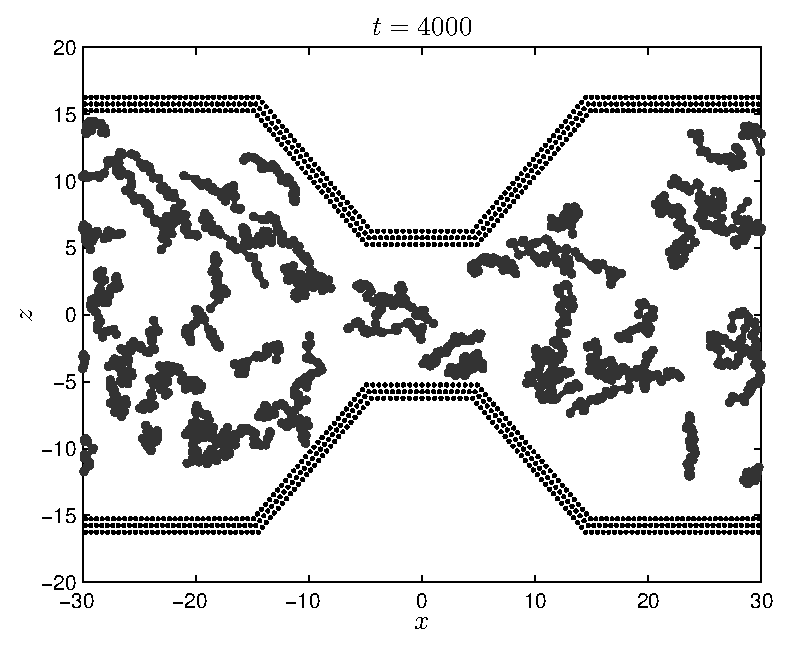
\includegraphics[width=7.5cm]{./figures/chainY4000s.eps}
\end{minipage}
\small nChain = 60, ChainLen = 30\\
\caption{\label{chainY}\small 斜坡微缩通道中$t=0$和$t=4000$时刻高分子链分布图.}
\end{figure}

图\ref{chainY}显示的是斜坡微缩通道中布置60个长度为30的高分子链在$t=0$和$t=4000$ 时刻高分子链分布(为了方便观察,简单流体粒子已经略去)。初始时刻高分
子链大致均匀分布,处于折叠状态。在$t=4000$时刻,与方型微缩通道(图\ref{chainT})相比, 斜坡微缩通道中高分子链能够得到更好伸展,但是与微直通道(图\ref{chain=})相比,高分子链伸展
还不够充分。图\ref{chainYprof}显示的是斜坡微缩通道有无高分子链两种情况在4000 时刻不同截面沿高度方向($z$)水平($x$)速度,温度及密度分布。比较
图\ref{chainYprof}(a)和图\ref{chainYprof}(b),可以得到与算例4.2类似的结论,这是由于本算例与算
例4.2不仅具有相同体积和相似形状的流动区域,还具有相同长度和数量
的高分子链。

\begin{figure}[!htb]
\centering
\begin{minipage}[c]{0.5\textwidth}
\centering
\includegraphics[width=7.5cm]{./figures/Yprof.eps}\\
\small (a) 无高分子链
\end{minipage}%
\begin{minipage}[c]{0.5\textwidth}
\centering
\includegraphics[width=7.5cm]{./figures/chainYprof.eps}\\
\small (b) 有高分子链
\end{minipage}
\caption{\label{chainYprof}\small 斜坡微缩通道不同截面沿高度方向($z$)水平($x$)速度,温度及密度分布.}
\end{figure}

尽管图\ref{chainYprof}显示的斜坡微缩通道在系统温度,粒子密度及水平速度表现出的性质与方形微缩通道较
为相似,但由于两种通道在结构上存在差异,其表现出的性质存在明显的差别。比较图\ref{chainTprof}和
图\ref{chainYprof}:无论有无高分子,方形微缩通道在不同截面的水平速度比斜坡微缩通道在相应截面上的
小,这是由于斜坡微缩通道相对于方形微缩通道有较缓的斜坡过度,对系统的流动减弱作用较
小;方形微缩通道在 $x=16.5$截面出现了回流,而斜坡微缩通道没有出现,这同样是由于方形微缩通道没
较缓的斜坡过度而引起的回流;对于方形微缩通道,水平速度在$x=-25.5$和$x=-16.5$截面处的分布有明
显差异,而对于斜坡微缩通道,则没有太明显差异,两条速度曲线几乎重合,这是由于斜坡微
缩通道相对于方形微缩通道有较缓的斜坡过度,速度在$x=-16.5$截面处没有太急剧的变化,因此
斜坡微缩通道水平速度在$x=-25.5$和$x=-16.5$截面处的分布没有明显差异。

\section{ 结论}

本文应用耗散粒子动力学方法与有限拉伸非线性弹性珠簧链模型,对微直通道
与微缩通道中DNA高分子输运与迁移的动态行为进行了数值模拟和分析研究。
通过对不同数量和长度的高分子链在微直通道及微缩通道中的流动行为的对比
研究,分析了系统的速度,温度及密度与高分子链数量、长度间的关系。研
究表明,与简单流体粒子在微直通道和微缩通道中流动相比,DNA分子的运动展
现出了明显的特点,高分子链的伸展状态与通道的形状密切相关。微直通道中
高分子链能得到充分伸展,高分子也主要集中在通道中心部位。方形微缩通
道中高分子链未能得到充分伸展,而斜坡微缩通道中高分子链的伸展状态则
介于直通道与方形微缩通道之间。高分子链的存在对系统的温度平衡及分布
没有明显影响,对沿高度方向的水平速度及密度则有较明显影响,高分子链
的存在会``拖累''周围的普通流体粒子,降低其周围流体粒子的流动速度,引
起局部粒子密度波动,形成比较明显的拖曳现象。微通道结构上细微的差别
也会对系统的流动特性产生明显的差异,这些差异主要表现在水平速度和粒子密度分布上。




\centerline{\hbox to 8cm{\hrulefill}}

\begin{thebibliography}{999}
\itemsep=-4pt plus.2pt minus.2pt  %% 用此参数调整参考文献条与条之间的间距
\small
\bibitem{Rapaport}  Rapaport D C 2004 \textit{The Art of Molecular Dynamics Simulation} (Cambridge, UK: Cambridge University Press)
\bibitem{Hoogerbrugge}	Hoogerbrugge P J, Koelman J 1992 \textit{Europhys. Lett.} \textbf{19} 155
\bibitem{Groot1997}	Groot R D 1997 \textit{J. Chem. Phys.} \textbf{107} 4423
\bibitem{Chen_S}  Chen S, Zhao J, Fan X J, Wang D 2006 \textit{Bull. Sci. Tech.} {\bf 22} 596 (in Chinese) [陈硕、赵钧、  范西俊、王丹 2006 \textit{科技通报} {\bf 22} 596]
\bibitem{Fan_X} Fan X,  Phan-Thien N,  Yong N T,  Wu X, Xu D 2003 \textit{Phys. Fluids} {\bf 15}
016201
\bibitem{Groot2003} Groot R D 2003 \textit{J. Chem. Phys.} {\bf 118} 11265
\bibitem{Groot2000} Groot R D 2000 \textit{Langmuir} {\bf 16} 7493
\bibitem{Dzwinel_W} Dzwinel W,  Yuen D A, Boryczko K 2002 \textit{J. Mol. Model.} {\bf 8} 33
\bibitem{Tanaka_H}	Tanaka H, Araki T 2000 \textit{Phys. Rev. Lett.} {\bf 85} 1338
\bibitem{Schlijper}	Schlijper A G,  Hoogerbrugge P J, Manke C W 1995 \textit{J. Rheol.} {\bf 39} 567
\bibitem{Venturoli} Venturoli M, Smit B 1999 \textit{PhysChemComm} {\bf 2} 45

\bibitem{MBLiu2006} Liu M B,  Meakin P, Huang H 2006 \textit{Phys. Fluids} {\bf 18} 017101
\bibitem{MBLiu2007wrr} Liu M B,  Meakin P, Huang H 2007 \textit{Water Resour. Res.} {\bf 43} doi:10.1029/2006WR004856
\bibitem{MBLiu2007jcp} Liu M B,  Meakin P, Huang H 2007 \textit{J. Comput. Phys.} {\bf 222} 110
\bibitem{MBLiu2008} Chang J Z, Liu M B, Liu H T 2008 \textit{Acta Phys. Sin.} {\bf 57} 3954 (in Chinese) [常建忠、刘谋斌、刘汉涛 2008 \textit{物理学报} {\bf 57} 3954]

\bibitem{Larson} Larson R. G. 1999 \textit{The Structure and Rheology of Complex
Fluids} (Oxford, UK: Oxford University Press)

\bibitem{H_Pan} H. Pan, T.Y. Ng., Hua Li, E. Moeendarbary 2010
\textit{Sensors and Actuators A} {\bf 157} 328


\bibitem{GRLiu} Liu G R, Liu M B 2003 \textit{Smoothed Particle Hydrodynamics: A Meshfree Particle Method} (Singapore: World Scientific)
\bibitem{Espanol} Espanol P, Warren P 1995 \textit{Europhys. Lett.} {\bf 30} 191

\end{thebibliography}

\end{document}





%%
%%图形插入指令\,1, 与\,\verb+\usepackage{graphicx}+\,配合使用, 指令形式:
%%
%%\begin{verbatim}
%%\includegraphics[选择变量]{被插入图形文件的文件名(包括eps扩展名)}
%%\end{verbatim}
%%
%%%% \includegraphics[选择变量]{被插入图形文件的文件名(包括eps扩展名)}
%%
%%各常用变量的解释请参见文本文件的注释.
%%%% 常用选择变量有:
%%%% width 图形宽度, 如 width=7cm
%%%% height 图形高度,如 height=8cm
%%%% angle  图形旋转角度 如 angle=60
%%%% scale  图形缩放因子(不带单位) scale=1.2
%%
%%\vspace*{4mm}
%%
%%%\centerline{\includegraphics{Fig.-1(file).eps}}  %%% 图形插入指令形式
%%
%%\begin{center}
%%\small 图~1 \  图注内容.
%%\end{center}
%%如果图注的内容较长需要分行排,则需使用指令:
%%
%%\begin{verbatim}
%%      \begin{center}
%%      \parbox{15.5cm}{\small{图~1 }  图注内容. }
%%      \end{center}
%%\end{verbatim}
%%这里段落盒子指令\,\verb+\parbox{15.5cm}+\,用\,15.5~cm\,的宽度参数是单栏排图形的宽度, 如果是双
%%栏排的图形,其宽度参数只能取\,7.5~cm\,以下. 请注意\,\verb+\parbox{15.5cm}+\,指令与下面排三线
%%表中使用的\,\verb+\begin{minipage}{15.5cm} ...... \end{minipage}+\,小页环境等效, 只不过前者使
%%用时需注意括号的配对,而后者使用起来相对简单一些.
%%
%%图形插入指令\,2, 与\,\verb+\usepackage{epsfig}+\,配合使用\,(这是早期的图形插入指令形式,现在
%%已不太有人使用), 指令形式:
%%
%% \verb+\centerline{\epsfig{file=Fig-2.eps,width=7cm,height=8cm,clip=}}+
%%
%%各常用变量的解释请参见文本文件的注释.
%%%% 常用输入变量有:
%%%% file 或 figure,图形文件名,如:file=fig-2.eps 或 figure=fig-2.eps
%%%% width 图形宽度, 如 width=7cm
%%%% height 图形高度,如 height=8cm
%%%% angle  图形旋转角度 如 angle=60
%%%% clip=  是一个在等号后不需赋值的参数,可保证图形不会越出由图形eps文件中BoundingBox 指定的边界
%%
%%%% 使用形式:
%%\vspace*{4mm}
%%
%%%\centerline{\epsfig{file=Fig-2.eps,width=7cm,height=8cm,clip=}} %%%%% 图形插入指令形式
%%
%%\begin{center}
%%\small 图~2 \   图注内容.
%%\end{center}
%%图注单、双栏排的处理规则同上.
%%
%%
%%表格插入形式:
%%\begin{center}
%%\tabcolsep=6pt  %%% 此参数用于调整表的整体宽度
%%\small
%%\renewcommand\arraystretch{1.1}  %% 调整表内行与行之间的纵向距离
%%%\begin{minipage}{15.5cm}{
%%\small 表~1 \  表注内容.
%%%\end{minipage}
%%\vglue5pt
%%\begin{tabular}{ c  c  c  l  r  c  c }  %% 指定一个有6列数据的表,c为列居中, l为列左对齐, r为列右对齐
%%\hline %% 表横线
%% 表头 & $x$ & $y$ & $z$ & $\alpha$ & $\beta$ & $\omega$ \\
%% \hline
%%  $a$ & {11} & {22} & {33} & {44} & {55} & {66} \\   %% 第1行
%%  $b$ & {21} & {22} & {23} & {24} & {25} & {26} \\   %% 第2行  %%%% 依次往下排其他行
%%\hline
%%\end{tabular}
%%\end{center}
%%如果表注的内容比较长需分行, 则需根据单双栏的情况按上面处理图注的原则处理. 如使用以下形式:
%%
%%\begin{verbatim}
%%\begin{center}
%%\tabcolsep=6pt  %%% 此参数用于调整表的整体宽度
%%\small
%%\renewcommand\arraystretch{1.1} %% 此参数用于调整表内行与行之间的纵向距离
%%\begin{minipage}{15.5cm} \small 表~1 \  表注内容.
%%\end{minipage}
%%\vglue5pt
%%\begin{tabular}{c c c l r c c} %% 指定一个有7列数据的表,c为列居中, l为列左对齐, r为列右对齐
%%\hline % 表横线
%% 横表头 & $x$ & $y$ & $z$ & $\alpha$ & $\beta$ & $\omega$ \\
%% \hline
%%  $a$ & {11} & {22} & {33} & {44} & {44} & {66} \\   %% 第1行
%%  $b$ & {21} & {22} & {23} & {24} & {25} & {26} \\   %% 第2行
%%  %%%% 依次往下排其它行
%%\hline
%%\end{tabular}
%%\end{center}
%%\end{verbatim}
%%即由给定的\,\verb+\begin{minipage}{15.5cm} ...... \end{minipage}+\,小页环境的宽度参数决定表
%%注的宽度和表的宽度,一般情况下,通栏\,(即单栏)表通常给\,15.5~cm\,的宽度参数, 双栏表通常
%%给\,7.5~cm\,以下的宽度参数.
%%
%%\vspace*{2mm}
%%
%%参考文献排版使用的环境格式:
%%\begin{verbatim}
%%\begin{thebibliography}{999}
%%\itemsep=-4pt plus.2pt minus.2pt  %% 调整参考文献条与条之间的间距
%%\small
%%\bibitem{1}  %% 输入参考文献1内容
%%\bibitem{2}  %% 输入参考文献2内容
%%\bibitem{3} %% 输入参考文献3内容,其余依次往下排
%%\end{thebibliography}
%%\end{verbatim}
%%
%%
%%\centerline{\hbox to 8cm{\hrulefill}}
%%
%%
%%\begin{thebibliography}{999}
%%\itemsep=-4pt plus.2pt minus.2pt  %% 用此参数调整参考文献条与条之间的间距
%%\small
%%\bibitem{1}  Rapaport D C 2004 \textit{The Art of Molecular Dynamics Simulation} (Cambridge, UK: Cambridge University Press)
%%\bibitem{2}  Groot R D 1997 \textit{J. Chem. Phys.} {\bf 107} 4423
%%\bibitem{3}  Chen S, Zhao J, Fan X J, Wang D 2006 \textit{Bull. Sci. Tech.} {\bf 22} 596 (in Chinese) [陈硕、赵钧、  范西俊、王丹 2006 \textit{科技通报} {\bf 22} 596]
%%\bibitem{4} Fan X,  Phan-Thien N,  Yong N T,  Wu X, Xu D 2003 \textit{Phys. Fluids} {\bf 15}
%%016201
%%\bibitem{5} Groot R D 2003 \textit{J. Chem. Phys.} {\bf 118} 11265
%%\bibitem{6} Groot R D 2000 \textit{Langmuir} {\bf 16} 7493
%%\bibitem{7} Dzwinel W,  Yuen D A, Boryczko K 2002 \textit{J. Mol. Model.} {\bf 8} 33
%%
%%
%%\bibitem{8}	Tanaka H, Araki T 2000 \textit{Phys. Rev. Lett.} {\bf 85} 1338
%%\bibitem{9}	Schlijper A G,  Hoogerbrugge P J, Manke C W 1995 \textit{J. Rheol.} {\bf 39} 567
%%\bibitem{10} Venturoli M, Smit B 1999 \textit{PhysChemComm} {\bf 2} 45
%%\bibitem{11} Liu M B,  Meakin P, Huang H 2006 \textit{Phys. Fluids} {\bf 18} 017101
%%\bibitem{12} Liu M B,  Meakin P, Huang H 2007 \textit{Water Resour. Res.} {\bf 43} doi:10.1029/2006WR004856
%%\bibitem{13} Liu M B,  Meakin P, Huang H 2007 \textit{J. Comput. Phys.} {\bf 222} 110
%%\bibitem{14} Chang J Z, Liu M B, Liu H T 2008 \textit{Acta Phys. Sin.} {\bf 57} 3954 (in Chinese) [常建忠、刘谋斌、刘汉涛 2008 \textit{物理学报} {\bf 57} 3954]
%%\bibitem{15} Liu G R, Liu M B 2003 \textit{Smoothed Particle Hydrodynamics: A Meshfree Particle Method} (Singapore: World Scientific)
%%\bibitem{16} Liu M B,  Meakin P, Huang H 2006 \textit{Phys. Fluids} {\bf 18} 017101
%%
%%\bibitem{Espanol} Espanol P, Warren P 1995 \textit{Europhys. Lett.} {\bf 30} 191
%%
%%\end{thebibliography}
%%
%%其中环境指令\,\verb+\begin{thebibliography}{999}+\,中取样参数\,\verb+{999}+\,的作
%%用是
%%决定\,[10]\,以上和\,[10]\,以下的参考文献序号的对齐方式\,(即左对齐还是右对齐), 可根据实际需要
%%适当增减数字个数\,(使用\,0, 1, 2, $\cdots\cdots$, 9\,之间的任何数字都可).
%
%
